\documentclass[10pt,twocolumn,letterpaper]{article}
\usepackage[margin=0.7in,columnsep=0.25in]{geometry}
\usepackage[T1]{fontenc}
\usepackage{lmodern}
\usepackage{mathptmx}
\usepackage{graphicx,booktabs,tabularx,xcolor,cite,microtype,enumitem,amsmath}
\usepackage[hidelinks]{hyperref}
\usepackage[font=small,labelfont=bf]{caption}
\usepackage{titlesec}
\usepackage{float}
\usepackage{pgfplots}
\pgfplotsset{compat=1.17}

\renewcommand\thesection{\Roman{section}}
\renewcommand\thesubsection{\Alph{subsection}}
\titleformat{\section}{\centering\normalsize\scshape}{\thesection.}{0.5em}{}
\titleformat{\subsection}{\normalsize\itshape}{\thesubsection.}{0.5em}{}
\titlespacing*{\section}{0pt}{8pt}{4pt}
\titlespacing*{\subsection}{0pt}{6pt}{3pt}
\setlist{nosep,leftmargin=1.2em}
\newcommand{\code}[1]{\texttt{\small #1}}

\title{\Large\bfseries Apache HBase Under Failure: Architecture, Consistency,\\Consensus and Chaos Testing of a Distributed Wide-Column Store}
\author{Team 3 \\ INFT 6000: Principles of Distributed Systems, Fall 2026}
\date{}

\begin{document}
\maketitle

\begin{abstract}
Apache HBase is an open-source wide-column store modelled on Google's Bigtable. It runs on top of HDFS and uses ZooKeeper for coordination. This report analyses how HBase distributes data, which consistency it guarantees and why, which consensus mechanisms keep the cluster correct, and how it behaves when nodes crash or are partitioned from the network. We built a 13-node cluster in Docker Compose: 3 ZooKeeper servers, an HDFS NameNode with 3 DataNodes, 2 HMasters, 3 RegionServers and a Thrift gateway. On it we measured the cost of write-ahead-log durability and of strong versus timeline-consistent reads, and we injected five kinds of fault while client traffic was running. HBase behaves as a CP system. When a RegionServer fails, only the regions it hosted stop accepting writes, for roughly the ZooKeeper session timeout plus the recovery time, and no acknowledged write was lost in any experiment. Timeline-consistent region replicas kept reads available during these windows at the cost of returning stale data, which is the PACELC trade-off made per request.
\end{abstract}

\section{Introduction}
NoSQL systems differ less in their data models than in how they answer one question: what happens when part of the cluster stops responding? Dynamo-style stores such as Cassandra keep accepting writes on any replica and reconcile later~\cite{dynamo}. HBase does the opposite. Every piece of data has exactly one server responsible for it at any moment, so reads are never stale, but that data is unavailable while ownership is moved after a failure.

HBase follows the Bigtable design~\cite{bigtable}. A table is a sorted map from row key to columns, split into contiguous key ranges called \emph{regions}, and each region is served by one RegionServer. Durability is delegated to HDFS~\cite{hdfs}, and cluster membership and leadership are delegated to ZooKeeper~\cite{zookeeper}. Consensus therefore happens in ZooKeeper's Zab protocol~\cite{zab}, not inside HBase. HBase builds a single-leader-per-region protocol on top of it, using leases (ZooKeeper sessions and HDFS file leases) for fencing.

Our contributions are:
\begin{itemize}
\item an analysis of HBase's topology, consistency, coordination and failure handling, organized around \emph{who is allowed to write a region and how that permission is fenced};
\item a reproducible 13-container HBase/HDFS/ZooKeeper cluster with a Python workload that exposes per-request durability and consistency levels;
\item five fault-injection experiments under live traffic, each followed by an automatic check that no acknowledged write was lost;
\item measurements of the cost of WAL durability, the replication lag of read replicas, and the unavailability window after crashes and partitions.
\end{itemize}

This report covers the four required areas: topology and data distribution (Sec.~\ref{sec:topo}), consistency (Sec.~\ref{sec:cons}), consensus and coordination (Sec.~\ref{sec:consensus}) and fault tolerance (Sec.~\ref{sec:ft}). It then presents our cluster (Sec.~\ref{sec:setup}) and the measurements and chaos experiments (Sec.~\ref{sec:results}). All code, configuration and scripts are in the team repository.

\section{Architectural Topology and Data Distribution}\label{sec:topo}

\subsection{Components}
Table~\ref{tab:roles} lists the processes of an HBase deployment, and Fig.~\ref{fig:arch} shows how they connect in our cluster. HBase has two planes:
\begin{itemize}
\item \textbf{Data plane:} clients talk directly to RegionServers. The HMaster is \emph{not} on the read/write path.
\item \textbf{Control plane:} the active HMaster assigns regions to RegionServers, balances load, executes DDL and runs crash recovery.
\end{itemize}
Because of this split, losing the master for a short time does not interrupt traffic. Our experiment in Sec.~\ref{sec:results} confirms this.

\begin{table}[t]
\caption{Processes in an HBase cluster and their responsibility}\label{tab:roles}
\small
\begin{tabularx}{\columnwidth}{@{}lX@{}}
\toprule
Process & Responsibility \\
\midrule
ZooKeeper (3) & Replicated coordination store: active-master lock, live RegionServers, location of \code{hbase:meta}. \\
HMaster (1 active + backups) & Region assignment, load balancing, schema changes, crash recovery through the procedure framework. \\
RegionServer ($n$) & Serves regions: WAL, MemStore, block cache, flushes and compactions. \\
HDFS NameNode & File namespace, block locations, file leases. \\
HDFS DataNodes & Store block replicas (default 3) of WAL files and HFiles. \\
\bottomrule
\end{tabularx}
\end{table}

\begin{figure*}[t]
\centering
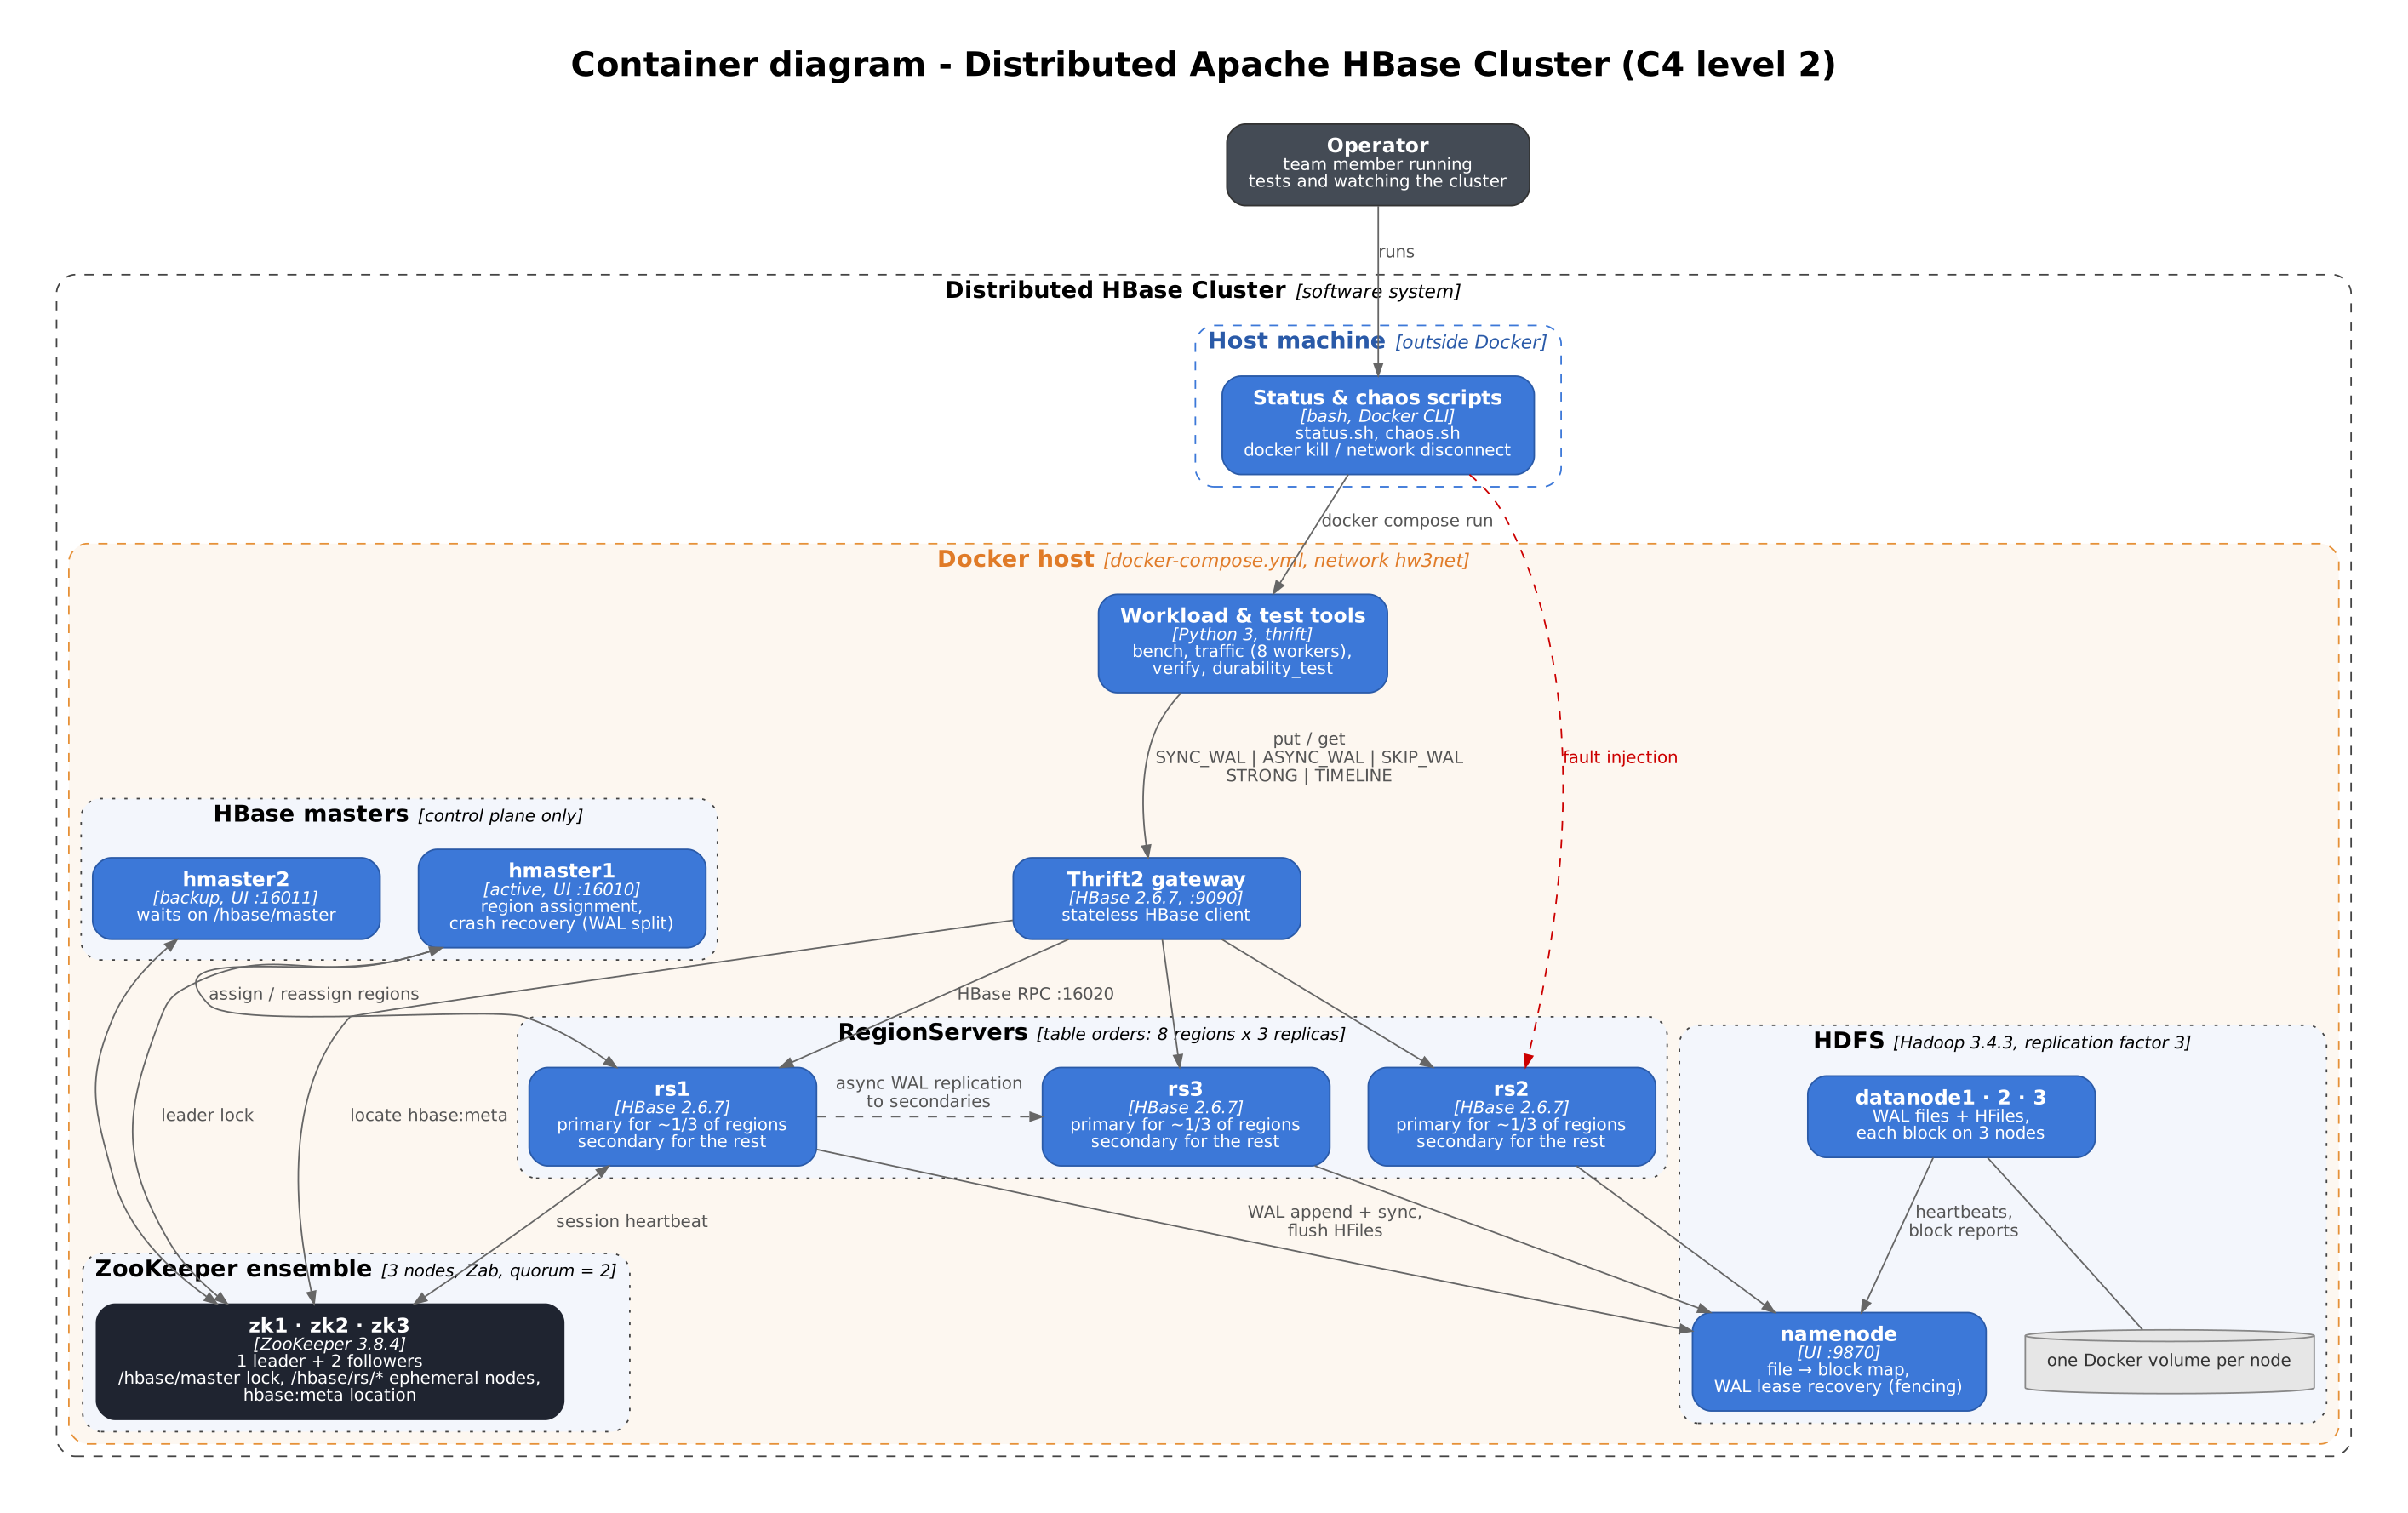
\includegraphics[width=0.86\textwidth]{fig/architecture.png}
\caption{C4 container diagram of our deployment (\code{docs/architecture.dot}). Clients reach RegionServers through a Thrift2 gateway. RegionServers keep their state on HDFS, and ZooKeeper tracks which servers are alive and which master is active.}\label{fig:arch}
\end{figure*}

\subsection{Data model}
An HBase table is a sparse, sorted, multi-dimensional map: (row key, column family, qualifier, timestamp) $\rightarrow$ value. Column families are declared in the schema and stored separately. Qualifiers are free-form and created on write. Table~\ref{tab:row} shows one row of our \code{orders} table. A row exists only where cells exist, so empty columns cost nothing, and every cell keeps up to \code{VERSIONS} timestamped values (1 in our table).

\begin{table}[t]
\caption{One row of table \code{orders} (column family \code{d})}\label{tab:row}
\small
\begin{tabularx}{\columnwidth}{@{}lllX@{}}
\toprule
Row key & Column & Timestamp & Value \\
\midrule
\code{a-o00000013} & \code{d:status} & 1795040123456 & \code{NEW} \\
                   & \code{d:amount} & 1795040123456 & \code{13} \\
                   & \code{d:ts}     & 1795040123456 & \code{1795040123.4} \\
\bottomrule
\end{tabularx}
\end{table}

\subsection{Sharding: range partitioning into regions}
HBase uses \emph{range partitioning}, not hashing. Rows are stored sorted by key, and a region holds the half-open interval $[\textit{startKey}, \textit{endKey})$. A new table has one region unless it is pre-split. A region splits in two when it grows past a threshold: HBase 2's default \code{SteppingSplitPolicy} splits small tables early (at twice the MemStore flush size) and later at \code{hbase.hregion.max.filesize} (10\,GB)~\cite{refguide}. The master then assigns the two daughters, and the balancer may move one of them to another server.

Clients find regions through a two-level lookup:
\begin{enumerate}
\item read the location of the catalog table \code{hbase:meta} from the ZooKeeper znode \code{/hbase/meta-region-server};
\item read the row of \code{hbase:meta} that covers the wanted key, which gives the hosting RegionServer;
\item send the request to that RegionServer directly.
\end{enumerate}
Locations are cached in the client. A stale cache entry is detected when a server answers \code{NotServingRegionException}, and the client then looks up the region again.

Range partitioning keeps rows sorted, so scans are efficient, but it causes \emph{hot-spotting} when keys are monotonic: all new timestamps or sequence numbers land in the last region. We avoid this with \emph{salting}. Our row key is \code{<salt>-<order id>}, where the salt is one of \code{0,2,4,6,8,a,c,e} chosen by \code{order\_id mod 8}. The table is pre-split at \code{2,4,6,8,a,c,e}, so consecutive orders go to eight different regions. The cost is that a range scan over order ids must fan out to all eight salt buckets.

\subsection{Inside a region: the storage engine}
Within a region, every column family is a separate \emph{store}: one MemStore in memory plus a set of immutable HFiles on HDFS. HFiles are sorted, block-indexed files with optional Bloom filters, and their blocks are cached in the RegionServer's block cache. The design is a log-structured merge tree~\cite{lsm}:
\begin{itemize}
\item writes are cheap because they only append to the WAL and insert into the sorted MemStore;
\item reads may need to merge the MemStore with several HFiles (read amplification). Bloom filters and the block cache keep this low;
\item \emph{minor compactions} merge a few small HFiles. \emph{Major compactions} rewrite all files of a store, dropping deleted and expired cells;
\item a region is the unit of distribution, so a split only creates two reference files that point into the parent's HFiles. The data is rewritten later by compaction, which makes a split almost instant.
\end{itemize}
Because HFiles live on HDFS, every RegionServer can read every region's files. Moving a region therefore moves \emph{ownership}, not data. This is why failover takes seconds rather than the time needed to copy gigabytes. The price is data locality: after a move, reads go over the network until compactions rewrite the files on the new host's local DataNode.

\subsection{Membership and failure detection}
HBase does not use gossip or SWIM. Membership is \emph{centralized in ZooKeeper}:
\begin{itemize}
\item Every RegionServer creates an \emph{ephemeral} znode \code{/hbase/rs/<host,port,startcode>}. The znode exists exactly as long as the server's ZooKeeper session.
\item The ZooKeeper client library heartbeats on the session. If the ensemble hears nothing for the session timeout (\code{zookeeper.session.timeout}, default 90\,s, set to 10\,s in our cluster), the session expires and the znode is deleted.
\item The active master watches \code{/hbase/rs}. A deleted child means a dead server, and the master starts a \code{ServerCrashProcedure} (Sec.~\ref{sec:ft}).
\item RegionServers also report load to the master every 3\,s (\code{hbase.regionserver.msginterval}). These reports carry statistics but are not the failure detector.
\end{itemize}
The \emph{startcode}, the server's start timestamp, makes each process incarnation unique. A restarted server on the same host and port is a new member, and the old incarnation can be recognised and rejected. HDFS has its own detector: DataNodes heartbeat to the NameNode every 3\,s and are declared dead after 10.5 minutes by default~\cite{hdfs}.

The failure detector therefore has a single tunable: a short session timeout gives fast recovery but risks false positives during long garbage-collection pauses. A falsely suspected server is still safe because of fencing (Sec.~\ref{sec:consensus}).

\section{Consistency Model Analysis}\label{sec:cons}

\subsection{Default and supported consistency levels}
By default HBase is \textbf{strongly consistent} for single-row operations. Each row is served by one region, and each region by one RegionServer, which serializes all mutations of that row. A \code{Put}, \code{Delete}, \code{Increment} or \code{CheckAndMutate} on one row is atomic across all column families of the row. Once a write is acknowledged, every subsequent read of that row sees it. This holds for reads by any client, not only the writer, so it is stronger than read-your-writes~\cite{refguide}. HBase gives no multi-row transactions, except multi-row mutations confined to a single region.

Since version 1.0 HBase also offers \textbf{timeline consistency} for reads on tables with region replicas (\code{REGION\_REPLICATION} $>1$)~\cite{timeline,hbase10070}. A region then has one \emph{primary} replica, which takes all writes, and read-only \emph{secondary} replicas on other servers. The level is chosen per request:
\begin{itemize}
\item \code{Consistency.STRONG} (default): the read goes to the primary only.
\item \code{Consistency.TIMELINE}: the read goes to the primary first. If the primary has not answered within \code{hbase.client.primaryCallTimeout.get} (10\,ms), the client also asks the secondaries and keeps the first answer. If a secondary answered, \code{Result.isStale()} is \code{true}.
\end{itemize}
A secondary sees edits in the same order as the primary, because they come from the primary's WAL, but possibly later. This is why the model is called \emph{timeline}: a reader may be behind on the timeline, but never sees an order of events that did not happen. There is no session stickiness, so two consecutive timeline reads served by different secondaries can go backwards in time~\cite{timeline}.

\textbf{Example.} Suppose a client writes \code{status=NEW}, then \code{PAID}, then \code{SHIPPED} to one order, and secondary replica~1 lags by one edit. A \code{STRONG} read after the third write always returns \code{SHIPPED}. A \code{TIMELINE} read may return \code{SHIPPED} from the primary, or \code{PAID} with \code{stale=true} from the replica. It can never return \code{NEW} after \code{PAID} from the same replica, and never a value that was not written. Without stickiness, two timeline reads in a row can still observe \code{SHIPPED} and then \code{PAID}, if they are answered by different replicas.

\subsection{Write path and durability levels}
Fig.~\ref{fig:write} shows a write. The primary RegionServer
\begin{enumerate}
\item appends the edit, with a sequence id, to its write-ahead log (WAL), an HDFS file;
\item inserts the edit into the region's MemStore, a sorted in-memory buffer;
\item syncs the WAL;
\item advances the region's MVCC read point so that readers can see the edit;
\item acknowledges the write.
\end{enumerate}
The WAL sync pushes the edit through the HDFS replication pipeline, DN1$\rightarrow$DN2$\rightarrow$DN3, and waits for the acknowledgement of all three DataNodes~\cite{hdfs}. When a MemStore reaches the flush size (128\,MB by default) it is written out as an immutable HFile. Background compactions merge HFiles, which makes HBase a log-structured merge tree~\cite{lsm}.

\begin{figure}[t]
\centering
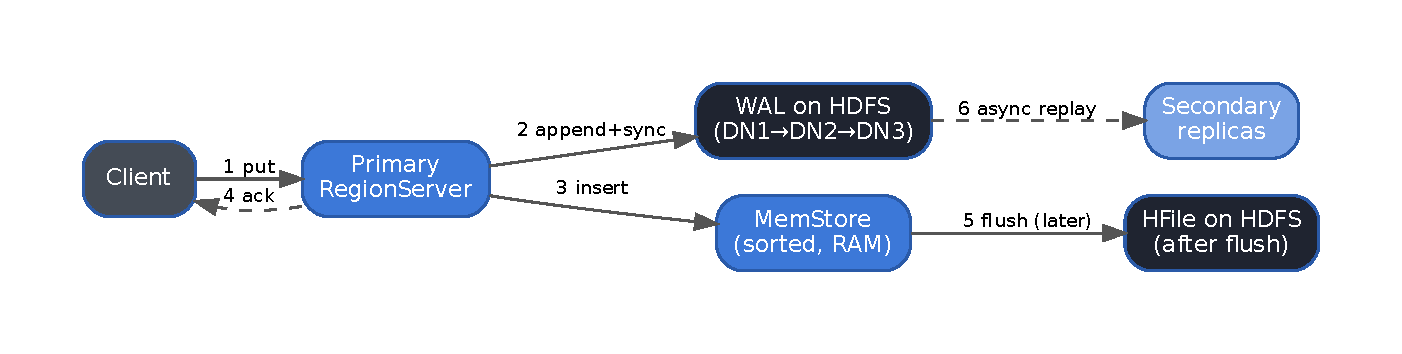
\includegraphics[width=\columnwidth]{fig/write_path.pdf}
\caption{Write path. The client is acknowledged after step 3 (WAL sync and MemStore). Flushes and replication to secondary replicas happen asynchronously.}\label{fig:write}
\end{figure}

Durability can be set per mutation or per table:
\begin{itemize}
\item \code{SKIP\_WAL}: no WAL. The edit lives only in the MemStore until a flush and is lost if the server crashes.
\item \code{ASYNC\_WAL}: acknowledge before the WAL is synced. A crash loses at most the last sync interval.
\item \code{SYNC\_WAL} (default): acknowledge after \code{hflush}, which means all three DataNodes have the bytes in memory.
\item \code{FSYNC\_WAL}: additionally \code{hsync} to disk on the DataNodes.
\end{itemize}
Note that \code{SYNC\_WAL} protects against a RegionServer crash and against the loss of up to two DataNodes. It does not protect against a simultaneous power loss of all three DataNodes, which is what \code{FSYNC\_WAL} is for. Section~\ref{sec:results} measures the latency of each setting and shows the data loss of \code{SKIP\_WAL} under a crash.

\subsection{Read path}
A \code{Get} merges three sources: the MemStore, the block cache, and the HFiles on HDFS, which are filtered with Bloom filters. Each read takes the region's current MVCC read point and ignores newer, not yet completed writes. Readers therefore never see a half-applied row mutation. Because only the primary accepts writes, a \code{STRONG} read at the primary always reflects every acknowledged write.

\subsection{Quorum view: $R + W > N$}
HBase is not a quorum system, but the quorum formula still explains its guarantees if we apply it at the right layer (Table~\ref{tab:quorum}). For serving, a region has $N{=}1$ owner, so reads and writes trivially overlap. For storage, HDFS writes the WAL to all $N{=}3$ replicas before acknowledging, so a reader of any single replica after recovery finds the data. Timeline reads are the only configuration where $R+W\le N$, and they are exactly the reads that are flagged stale.

\begin{table}[t]
\caption{Overlap condition at each layer}\label{tab:quorum}
\small
\begin{tabularx}{\columnwidth}{@{}Xcccc@{}}
\toprule
Layer / mode & $N$ & $W$ & $R$ & $R{+}W{>}N$ \\
\midrule
Region serving, \code{STRONG} & 1 & 1 & 1 & yes \\
HDFS WAL pipeline & 3 & 3 & 1 & yes \\
Region replicas, \code{TIMELINE} & 3 & 1 & 1 & no (stale possible) \\
ZooKeeper (Zab) & 3 & 2 & 1$^{*}$ & see Sec.~\ref{sec:consensus} \\
\bottomrule
\end{tabularx}
\footnotesize $^{*}$ZooKeeper reads are served by any server and can lag; \code{sync()} before a read makes it reflect all earlier writes.
\end{table}

\subsection{Conflict resolution and anti-entropy}
Dynamo-style stores need vector clocks or last-write-wins, read repair, hinted handoff and Merkle-tree anti-entropy, because several replicas accept writes concurrently and diverge~\cite{dynamo}. HBase avoids divergence by design: \emph{one writer per region}, so there are no concurrent conflicting versions to reconcile. The remaining mechanisms are:
\begin{itemize}
\item \textbf{Cell versions (LWW per cell).} Every cell carries a timestamp, and the newest timestamp wins on read. If two edits carry the same timestamp, the one with the higher sequence id wins. This is the only ``conflict rule'', and it is deterministic because one server assigns the sequence ids.
\item \textbf{WAL replay instead of read repair.} After a crash, the edits of the dead server's WAL are split per region and replayed before the region opens elsewhere (Sec.~\ref{sec:ft}). This ``reconciles'' the new owner with the old one.
\item \textbf{Storage-level anti-entropy in HDFS.} DataNodes send block reports to the NameNode, which re-replicates under-replicated blocks. Checksums detect and replace corrupt replicas.
\item \textbf{Region replica catch-up.} Secondaries receive the primary's edits through an internal replication peer that tails the WAL. Flush and compaction markers in the WAL tell them which HFiles to switch to. A secondary cannot flush on its own~\cite{timeline}.
\item \textbf{Operator repair.} Inconsistencies between \code{hbase:meta}, HDFS and the assignment state are repaired with HBCK2, not automatically.
\end{itemize}

\section{Consensus and Coordination Protocols}\label{sec:consensus}

\subsection{ZooKeeper and Zab}
HBase delegates agreement to ZooKeeper, which replicates a small hierarchical store with the Zab atomic broadcast protocol~\cite{zookeeper,zab}. An ensemble of $2f{+}1$ servers tolerates $f$ failures. Our 3 servers tolerate 1. Zab works in phases:
\begin{enumerate}
\item \textbf{Leader election.} After a leader failure, servers vote for the candidate with the most recent history, ordered by $\langle\textit{epoch}, \textit{zxid}, \textit{server id}\rangle$. A candidate supported by a quorum (2 of 3) becomes leader of a new epoch.
\item \textbf{Discovery and synchronization.} The new leader brings followers up to date with its history, so no committed transaction is lost.
\item \textbf{Broadcast.} Each write gets a zxid (epoch, counter), is proposed to the followers and is committed once a quorum has logged it. All servers apply writes in zxid order.
\end{enumerate}
Zab is close to Raft~\cite{raft}: one leader per epoch (term), quorum commit, and election restricted to up-to-date candidates. Split brain is impossible because two quorums of 3 always intersect. A leader cut off from the majority cannot commit and steps down, and the majority side elects a new leader with a higher epoch.

\subsection{What HBase builds on top}
\begin{itemize}
\item \textbf{Master election.} Masters race to create the ephemeral znode \code{/hbase/master}. The winner is active, and the others register under \code{/hbase/backup-masters} and watch the lock. When the active master's session ends, the znode disappears and a backup takes over. A new master rebuilds its state from \code{hbase:meta} and the procedure store on HDFS, then resumes unfinished procedures.
\item \textbf{Liveness of RegionServers.} Ephemeral znodes, as described in Sec.~\ref{sec:topo}.
\item \textbf{Region ownership (single leader per region).} In HBase 2 the assignment state is stored in \code{hbase:meta} and changed only by master procedures (AssignmentManager v2). Regions are therefore ``elected'' by the master, not by voting among RegionServers.
\end{itemize}

\subsection{Region state machine}
Every region moves through a small state machine owned by the master: \code{OFFLINE} $\rightarrow$ \code{OPENING} $\rightarrow$ \code{OPEN} $\rightarrow$ \code{CLOSING} $\rightarrow$ \code{CLOSED}, with extra states for split and merge. Each transition is a step of a \code{TransitRegionStateProcedure}, and each step is persisted in the master's procedure store before it is executed. If the master dies halfway through a move, the new master resumes the procedure from its last persisted step instead of guessing. Combined with the single active master, this gives a total order on all ownership changes, which is effectively a replicated state machine with one writer, made durable by HDFS.

\subsection{Split-brain prevention and fencing}
The difficult case is a RegionServer that is \emph{alive but unreachable}, for example because of a network partition or a long GC pause. The master declares it dead and reassigns its regions, but the old process may still believe it owns them. HBase prevents two writers per region with three layers of fencing:
\begin{enumerate}
\item \textbf{HDFS lease recovery.} Before splitting a dead server's WAL, the master renames its WAL directory and calls \code{recoverLease} on each WAL file. The NameNode closes the file and revokes the old writer's lease. Any further append or sync by the old server fails, so it can no longer acknowledge writes. This is the critical safety step.
\item \textbf{Session expiry.} When the isolated server reconnects to ZooKeeper, it learns that its session expired and aborts.
\item \textbf{YouAreDeadException.} If it contacts the master first, the master rejects the report from an expired server incarnation, identified by its startcode, and the server aborts.
\end{enumerate}
The same lease-recovery idea fences an old master: its procedure store lives in an HDFS-backed local region.

\section{Fault Tolerance and Partition Handling}\label{sec:ft}

\subsection{CAP and PACELC classification}
Under a partition HBase chooses consistency: regions owned by a server on the minority side become unavailable until they are reassigned. It never accepts writes on two sides. HBase is therefore \textbf{CP}~\cite{cap}. In PACELC terms~\cite{pacelc} it is \textbf{PC/EC} by default: even without failures, every \code{STRONG} read must reach the primary. Region replicas let a client move individual reads to \textbf{PA/EL}: with \code{TIMELINE} a read stays available during the failover window and can take the fastest replica, at the cost of staleness. Writes remain PC because they always go to the primary.

\subsection{Node failure: RegionServer crash, step by step}
\begin{enumerate}
\item $t_0$: the process dies. Writes and \code{STRONG} reads for its regions start failing or timing out. Other regions are unaffected.
\item $t_0$ + session timeout: ZooKeeper expires the session and deletes \code{/hbase/rs/<server>}. The master starts a \code{ServerCrashProcedure} (SCP).
\item If the server hosted \code{hbase:meta}, SCP first splits the meta WAL and reassigns meta. Until then, location lookups for all regions fail.
\item SCP renames the WAL directory to \code{-splitting} and recovers the HDFS leases (fencing).
\item The WALs are split into per-region \code{recovered.edits} files.
\item Each region is assigned to a live server, which replays its recovered edits, flushes, and opens the region. The master updates \code{hbase:meta}.
\item Clients get \code{NotServingRegionException} or connection errors, look up the new location and continue.
\end{enumerate}
Fig.~\ref{fig:scp} summarizes these steps. The unavailability window per region is roughly \emph{session timeout + WAL split + region open}. With secondary replicas, \code{TIMELINE} reads continue throughout. Secondaries are not promoted. The primary is reopened from HDFS, so the WAL remains the single source of truth.

\begin{figure}[t]
\centering
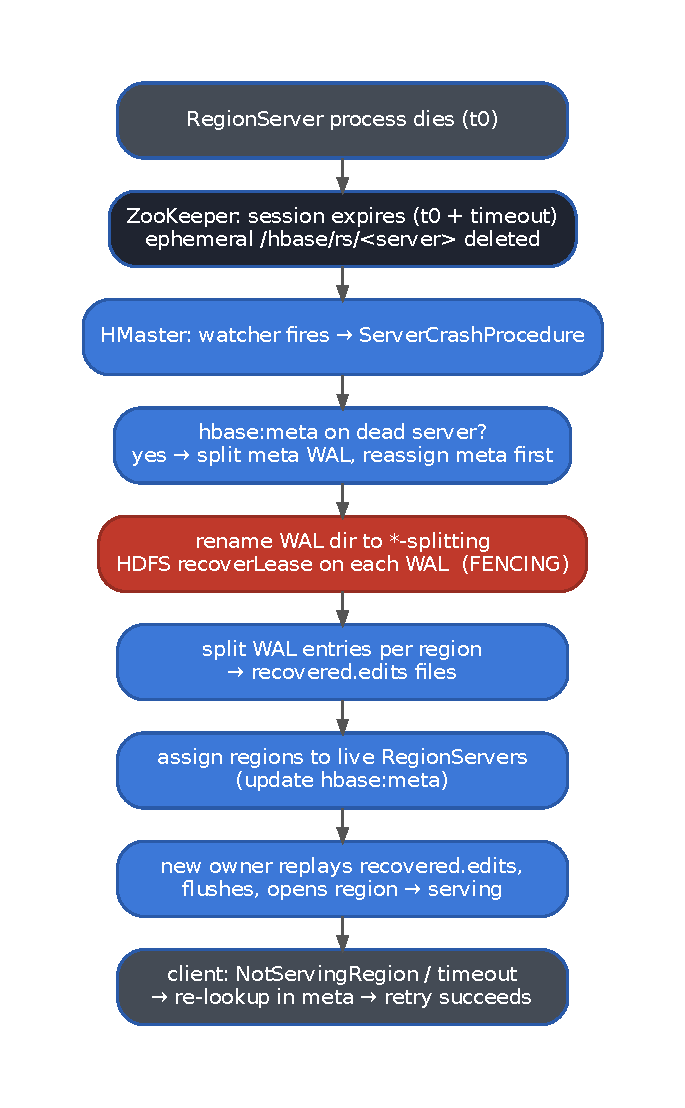
\includegraphics[height=0.42\textheight]{fig/scp.pdf}
\caption{ServerCrashProcedure. Lease recovery (red) is the step that fences the old server.}\label{fig:scp}
\end{figure}

\subsection{Network partition (split-brain scenario)}
If a RegionServer is isolated from the rest of the cluster:
\begin{itemize}
\item The majority side (ZooKeeper quorum, master, other RegionServers) cannot hear its heartbeats. Its session expires and SCP runs as above. The server is fenced by HDFS lease recovery, so even if a client on its side reached it, its WAL syncs would fail and nothing would be acknowledged.
\item The minority server cannot reach ZooKeeper either. When the partition heals, it sees the expired session or receives \code{YouAreDeadException} and aborts. It must be restarted, and it rejoins as a new incarnation with no regions.
\end{itemize}
Fig.~\ref{fig:fencing} shows both sides of this sequence. Sec.~\ref{sec:results} reports the timing we measured for it.

\begin{figure}[t]
\centering
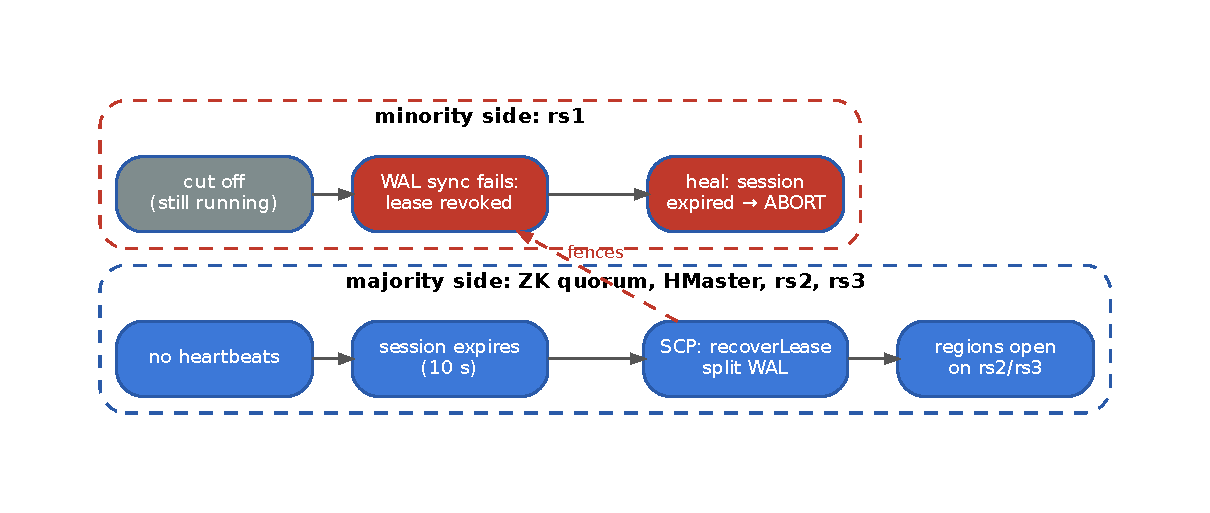
\includegraphics[width=\columnwidth]{fig/fencing.pdf}
\caption{Partition of one RegionServer. The majority side reassigns its regions and revokes its WAL lease, so the minority server can no longer acknowledge writes and aborts when it reconnects.}\label{fig:fencing}
\end{figure}

If a ZooKeeper server is on the minority side, it stops serving because it cannot form a quorum. Its clients reconnect to a majority server within their session timeout, so their sessions survive. If the \emph{active master} is isolated, its session expires, a backup becomes active, and the old master aborts when it notices the lost lock or a failed write to its store.

\subsection{Other membership changes}
\begin{itemize}
\item \textbf{Master failure:} a backup acquires \code{/hbase/master} after the session timeout. Data traffic continues. Only DDL, balancing and new crash recovery wait.
\item \textbf{ZooKeeper leader failure:} the followers re-elect, and the ensemble is unavailable for writes for the length of the election. HBase sessions survive if the election finishes within the session timeout.
\item \textbf{DataNode failure:} the WAL pipeline is rebuilt with the remaining nodes, or the WAL is rolled. The NameNode later re-replicates under-replicated blocks.
\item \textbf{Adding a RegionServer:} the new server registers its ephemeral znode and reports to the master. The \code{StochasticLoadBalancer}, which runs every 5 minutes or on the \code{balancer} command, moves regions to it. Each move closes the region (with a flush) on the source and opens it on the target, a sub-second outage per region.
\item \textbf{Decommissioning:} \code{decommission\_regionservers} marks a server as draining and moves its regions away one at a time. Unlike a crash, no WAL splitting is needed because regions are flushed and closed cleanly.
\end{itemize}

\section{Experimental Setup}\label{sec:setup}
\textbf{Cluster.} One Docker Compose file starts 13 long-running containers on one bridge network (Fig.~\ref{fig:arch}): ZooKeeper 3.8.4~$\times$3; Hadoop 3.4.3 NameNode and 3 DataNodes (replication factor 3); HBase 2.6.7 HMaster~$\times$2, RegionServer~$\times$3 and a Thrift2 gateway; and a one-shot job that creates the table. HDFS and HBase share one image built from the official Apache binaries on Eclipse Temurin Java 11. The ZooKeeper session timeout is 10\,s. Region replica replication is enabled.

\textbf{Table.} \code{orders}, one column family, pre-split into 8 regions, \code{REGION\_REPLICATION=3}. Each region therefore has a primary on one RegionServer and a secondary on each of the other two.

Table~\ref{tab:placement} shows where the replicas were placed when the experiments started. The balancer puts the three replicas of a region on three different servers, so every RegionServer hosts exactly one replica of every region: the primary of some regions and a secondary of the rest.

\begin{table}[t]
\caption{Region replica placement at the start of the experiments}\label{tab:placement}
\small
\begin{tabularx}{\columnwidth}{@{}Xccc@{}}
\toprule
Region (start key) & primary & replica 1 & replica 2 \\
\midrule
\code{-} (first) & rs3 & rs1 & rs2 \\
\code{2} & rs2 & rs3 & rs1 \\
\code{4} & rs1 & rs2 & rs3 \\
\code{6} & rs3 & rs1 & rs2 \\
\code{8} & rs3 & rs1 & rs2 \\
\code{a} & rs1 & rs2 & rs3 \\
\code{c} & rs1 & rs2 & rs3 \\
\code{e} & rs2 & rs3 & rs1 \\
\bottomrule
\end{tabularx}
\footnotesize \code{hbase:meta} was hosted on rs1, so the crash experiment chose rs3.
\end{table}

\textbf{Clients.} Python tools (\code{client/}) use the HBase Thrift2 API, which exposes per-request durability (\code{TPut.durability}), per-request consistency (\code{TGet.consistency}, \code{targetReplicaId}) and the \code{stale} flag. The gateway is itself an HBase client, configured to fail fast (3 retries, 4\,s operation timeout) so that outages are visible instead of being hidden by long retries.
\begin{itemize}
\item \code{bench.py}: write latency and throughput per durability mode, \code{STRONG} versus \code{TIMELINE} reads, and a freshness probe (write, then immediately read from secondary replica~1).
\item \code{traffic.py}: 8 worker threads, one per region, each doing a \code{SYNC\_WAL} write followed by a \code{STRONG} and a \code{TIMELINE} read, about 5 times per second. It prints a per-second line with a per-region map and logs every acknowledged key.
\item \code{verify.py}: re-reads every acknowledged key after the experiment.
\item \code{chaos.sh}: runs each fault scenario while \code{traffic.py} is active, using \code{docker kill} (crash) and \code{docker network disconnect} (partition).
\end{itemize}

\section{Results}\label{sec:results}
All numbers come from one end-to-end run of \code{scripts/selftest.sh} on a freshly created cluster (empty volumes). The host was an Apple-silicon MacBook (10 CPUs) running Docker Desktop with 8\,GB of memory. All 13 containers share this one machine, so absolute latencies are not representative of a real deployment. The \emph{differences} between settings and the \emph{timing} of failure handling are the meaningful results.

\begin{table*}[t]
\caption{HBase compared with Cassandra and MongoDB}\label{tab:compare}
\small
\begin{tabularx}{\textwidth}{@{}lXXX@{}}
\toprule
 & Apache HBase & Apache Cassandra & MongoDB (replica set / sharded) \\
\midrule
Partitioning & key ranges (regions), split on size & consistent hashing with virtual nodes & ranged or hashed chunks per shard \\
Writers per key & 1 (region primary) & any replica (leaderless) & 1 (shard primary) \\
Replication & below the database, in HDFS (3 copies of WAL and HFiles) & between database nodes, $N$ replicas & oplog shipped from primary to secondaries \\
Consensus & ZooKeeper (Zab) for membership and master; leases for regions & none for normal writes; Paxos for lightweight transactions & Raft-like election among data replicas \\
Default consistency & strong per row & tunable ($R{+}W{>}N$ with QUORUM) & primary reads, majority write concern \\
Conflict handling & none needed (single writer); timestamp per cell & last-write-wins, read repair, hinted handoff, Merkle trees & none needed; rollback of unreplicated writes after failover \\
Partition behaviour & CP: minority regions unavailable & AP at ONE, CP at QUORUM & CP: minority side has no primary \\
\bottomrule
\end{tabularx}
\end{table*}

\subsection{Baseline: durability and consistency settings}
Table~\ref{tab:bench} shows 2000 sequential operations per setting from one client, after a warm-up of 500 writes. Every request crosses the Python client, the Thrift gateway and the RegionServer, which costs about 0.4\,ms in total.

\begin{table}[t]
\caption{Latency and throughput per setting (one client, 2000 ops each)}\label{tab:bench}
\small
\begin{tabularx}{\columnwidth}{@{}Xrrrr@{}}
\toprule
Setting & ops/s & p50 ms & p95 ms & p99 ms \\
\midrule
Write \code{SKIP\_WAL}  & 1830 & 0.51 & 0.81 & 1.42 \\
Write \code{ASYNC\_WAL} & 2016 & 0.40 & 0.91 & 2.91 \\
Write \code{SYNC\_WAL}  & 1051 & 0.78 & 1.62 & 4.07 \\
\midrule
Read \code{STRONG}      & 1706 & 0.47 & 0.98 & 2.17 \\
Read \code{TIMELINE}    & 2261 & 0.40 & 0.65 & 0.97 \\
\bottomrule
\end{tabularx}
\end{table}

\textbf{Durability.} \code{SYNC\_WAL}, the default, halves throughput compared with the two asynchronous modes and adds about 0.3--0.4\,ms to the median and 1--3\,ms to the tail. This is the cost of waiting for the three-DataNode pipeline before acknowledging. \code{SKIP\_WAL} and \code{ASYNC\_WAL} are within measurement noise of each other, because neither waits for HDFS. What separates them is the failure behaviour shown in Sec.~VII-E, not their speed.

\textbf{Read consistency.} In a healthy cluster the primary always answers within the 10\,ms \code{primaryCallTimeout}, so all 2000 \code{TIMELINE} reads were served by the primary, and \emph{none} was stale. Both modes therefore take the same path, and the remaining gap is a warm-cache and ordering effect, not a property of the mode. Timeline consistency changes nothing while the system is healthy. It only matters during failures (Sec.~VII-B).

\textbf{Freshness of secondaries.} To isolate replication lag, we wrote a new value and immediately read it from secondary replica~1 (\code{targetReplicaId=1}). In all 100 probes the first read returned the old value, so the secondary was always behind. The new value appeared after a median of 2.0\,s (p95 4.9\,s, maximum 5.0\,s). Secondaries are updated by an asynchronous replication peer that tails the primary's WAL in batches. Their lag is therefore of the order of seconds, not milliseconds, which is why timeline reads must be treated as possibly stale.

A first attempt revealed a further detail. Before the primary had flushed even once, secondary replicas did not serve reads at all. HBase makes a secondary wait for a flush marker from the primary before it opens for reads (\code{hbase.region.replica.wait.for.primary.flush}). Our table-creation job therefore flushes the new table once.

\subsection{RegionServer crash}\label{sec:rscrash}
We killed \code{rs3}, which held the primaries of 3 of the 8 regions and did not host \code{hbase:meta}, with \code{docker kill}. Client traffic was running at 40 writes/s (Fig.~\ref{fig:rscrash}). Observed sequence:
\begin{itemize}
\item $t{=}20$\,s: crash. Within one second the three affected regions stopped answering. Workers writing to them blocked until the 4\,s client operation timeout and then reported failures. The other five regions continued at full rate, so total write throughput dropped from 40 to 25 ops/s and never to zero.
\item $t{=}21$--36\,s: \textbf{16 s of write unavailability} for the affected regions. This matches the 10\,s ZooKeeper session timeout plus about 5\,s for the master's \code{ServerCrashProcedure}: splitting the WAL, reassigning the regions and replaying the edits.
\item During this window, 12 \code{STRONG} reads failed. The \code{TIMELINE} reads of the same rows all succeeded, 13 of them with the stale flag set because a secondary answered.
\item $t{=}37$\,s: all eight regions were writable again on the two surviving servers. At $t{=}65$\,s \code{rs3} was restarted and rejoined with no regions, until the balancer moved some back.
\end{itemize}
\code{verify.py} re-read all 3750 acknowledged writes, and \textbf{none was lost}. The 15 failed writes were not present either, so each client-side timeout corresponded to a write that had not been applied.

\begin{figure*}[t]
\centering
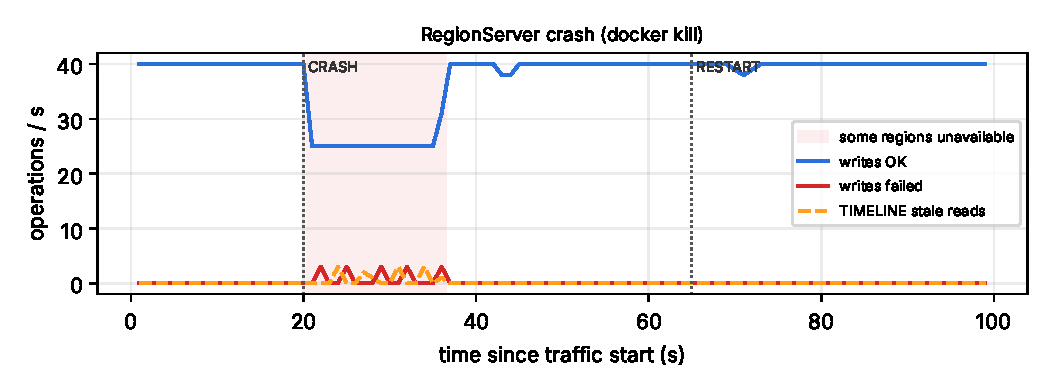
\includegraphics[width=0.8\textwidth]{fig/rs_crash.pdf}
\caption{RegionServer crash under load. The shaded area marks seconds in which at least one region was unavailable. Only the regions of the crashed server stop, and timeline reads stay available with stale results.}\label{fig:rscrash}
\end{figure*}

\subsection{Network partition}
We disconnected \code{rs1}, which held 4 primaries, from the Docker network for 50\,s (Fig.~\ref{fig:partition}). From the cluster's point of view this looks like a crash, and the timing was identical: \textbf{16 s} of unavailability for the four affected regions ($t{=}21$--36\,s), followed by reassignment. The isolated server could not reach ZooKeeper, the HMaster or the DataNodes. When the network was restored at $t{=}71$\,s, its ZooKeeper session had already expired and its WAL leases had been recovered by the master. The server therefore shut itself down instead of serving its old regions again, and the script restarted it as a new incarnation. No client ever saw two servers accept writes for the same region. Of 4463 acknowledged writes, \textbf{0 were lost}. 8 writes and 8 \code{STRONG} reads failed during the window, while \textbf{0 \code{TIMELINE} reads failed}. This run demonstrates the CP choice directly: the minority side loses availability, and the majority side stays consistent.

\begin{figure*}[t]
\centering
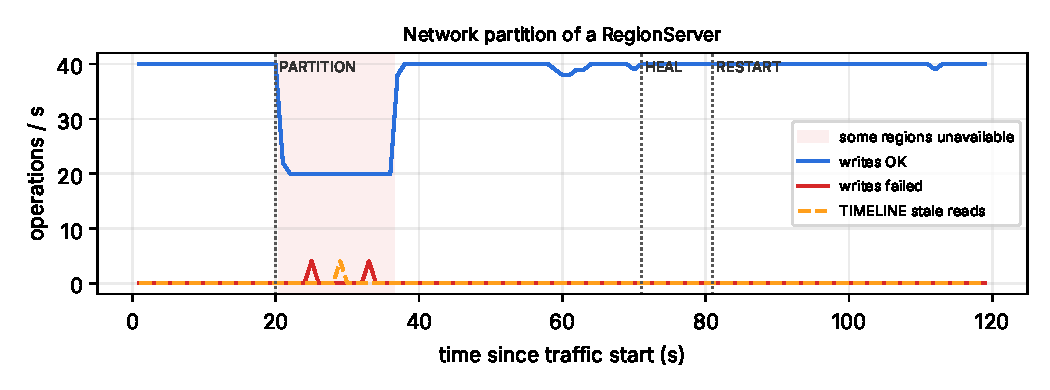
\includegraphics[width=0.8\textwidth]{fig/partition.pdf}
\caption{Network partition of one RegionServer. The isolated server is fenced and later restarts as a new instance. The data path recovers on the majority side after about 16\,s.}\label{fig:partition}
\end{figure*}

\subsection{Master failover and ZooKeeper leader failure}
Fig.~\ref{fig:control} shows both runs. \textbf{HMaster.} Killing the active \code{hmaster1} had \textbf{no effect on client traffic}: 2392 writes, 0 failures. Masters are not on the data path. Within the 26\,s observation window the backup \code{hmaster2} had acquired the \code{/hbase/master} lock and become active. The restarted \code{hmaster1} rejoined as backup.

\textbf{ZooKeeper.} Killing the ZooKeeper leader \code{zk3} triggered a Zab election, and five seconds later \code{zk2} was the new leader, with \code{zk1} as follower and \code{zk3} down. Traffic again saw \textbf{0 failures} out of 1792 writes. The two surviving servers still formed a quorum, and the clients' sessions moved to them before the 10\,s timeout. The restarted \code{zk3} rejoined as follower.

\begin{figure}[t]
\centering
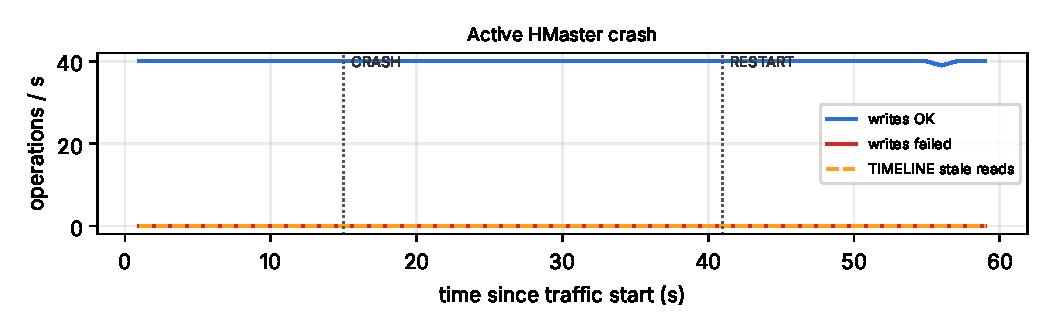
\includegraphics[width=\columnwidth]{fig/master.pdf}\\[2pt]
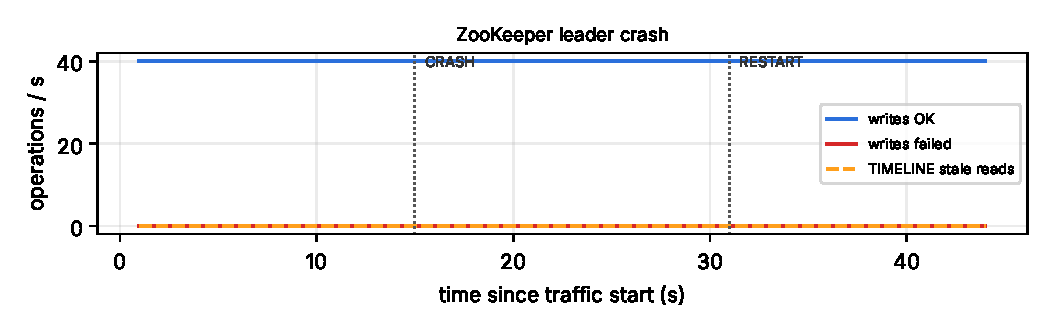
\includegraphics[width=\columnwidth]{fig/zk.pdf}
\caption{Control-plane failures: the active HMaster (top) and the ZooKeeper leader (bottom). Write throughput stays at 40 ops/s with no failures.}\label{fig:control}
\end{figure}

\subsection{What the WAL buys: crash with unflushed data}\label{sec:walloss}
We wrote 400 rows with \code{SKIP\_WAL} and 400 with \code{SYNC\_WAL}, spread over all regions, verified that all 800 were readable, and then killed \code{rs2} before any flush. Table~\ref{tab:walloss} shows the state after recovery. Every \code{SKIP\_WAL} row whose region was hosted on \code{rs2}, 50 rows in each of its 4 regions, disappeared. Those rows had existed only in that server's MemStore. Every \code{SYNC\_WAL} row survived, because the WAL on HDFS was split and replayed on the new servers. The durability setting is therefore a \emph{correctness} decision, not a performance tweak: \code{SKIP\_WAL} gained nothing measurable over \code{ASYNC\_WAL} in Table~\ref{tab:bench}, but loses every unflushed row on a crash.

\begin{table}[t]
\caption{Rows readable after a RegionServer crash before any flush}\label{tab:walloss}
\small
\begin{tabularx}{\columnwidth}{@{}Xrrr@{}}
\toprule
Durability & written & after recovery & lost \\
\midrule
\code{SKIP\_WAL} & 400 & 200 & 200 (4 regions $\times$ 50) \\
\code{SYNC\_WAL} & 400 & 400 & 0 \\
\bottomrule
\end{tabularx}
\end{table}

\subsection{Summary of fault experiments}
\begin{table}[t]
\caption{Fault experiments under live traffic (40 writes/s)}\label{tab:chaos}
\small
\begin{tabularx}{\columnwidth}{@{}Xrrrr@{}}
\toprule
Fault & unavail. & acked & failed & lost \\
\midrule
RegionServer crash (3/8 regions) & 16 s & 3750 & 15 & 0 \\
RegionServer partition (4/8) & 16 s & 4463 & 8 & 0 \\
Active HMaster crash & 0 s & 2392 & 0 & 0 \\
ZooKeeper leader crash & 0 s & 1792 & 0 & 0 \\
\bottomrule
\end{tabularx}
\footnotesize Unavailability applies only to the regions of the failed server. Other regions were unaffected. \code{TIMELINE} reads never failed in any experiment.
\end{table}

Table~\ref{tab:chaos} summarizes the four experiments. The results line up with the analysis in Sections~\ref{sec:cons}--\ref{sec:ft}:
\begin{enumerate}
\item failure detection is bounded by the ZooKeeper session timeout;
\item unavailability is limited to the regions of the failed server;
\item control-plane failures (master, ZooKeeper leader) do not interrupt the data path;
\item fencing prevents a partitioned server from coming back with stale ownership;
\item no acknowledged write is lost as long as the WAL is used.
\end{enumerate}

\section{Discussion}
\textbf{Tuning the detection window.} About two thirds of the 16\,s outage is the session timeout. We chose 10\,s, down from the 90\,s default. In production a lower value is risky: a garbage-collection pause longer than the timeout makes a healthy server look dead. Fencing keeps this safe, but it is expensive, because the server aborts and all its regions move. Operators therefore trade mean time to recovery against false suspicion. This is the same trade-off as the election timeout in Raft.

\textbf{When timeline reads are worth it.} Region replicas triple the memory used for MemStores and block caches, and they add replication traffic. In exchange, reads stay available through the outage window shown in Fig.~\ref{fig:rscrash}. They suit read-mostly workloads that tolerate seconds of staleness, such as product catalogs or dashboards. They do not suit read-modify-write logic, for which \code{STRONG} reads or \code{checkAndMutate} are required.

\textbf{Comparison with other systems.} Table~\ref{tab:compare} places HBase next to the two systems most often compared with it. Cassandra's leaderless design can stay writable on both sides of a partition and therefore needs the anti-entropy machinery that HBase does not have. MongoDB, like HBase, has one writer per shard, but it elects that writer with a Raft-like protocol among the data replicas themselves. HBase delegates election to ZooKeeper and durability to HDFS.



\textbf{Lessons from building the cluster.} Three problems we hit while building the environment taught us more about HBase than the documentation did:
\begin{itemize}
\item \emph{Identity matters.} RegionServers first aborted with ``Master passed us a different hostname''. The master had reverse-resolved a container's IP to \code{rs1.hw3net}, while the server called itself \code{rs1}. HBase treats a server's name, port and startcode as its identity, because that identity is what fencing and the dead-server list are keyed on. A mismatch is therefore fatal by design.
\item \emph{Secondaries are not readable on day one.} Timeline reads to a new table failed until the primary had flushed once, because a secondary waits for a flush marker before it trusts its own view.
\item \emph{Dead servers are remembered.} After the failed first starts, the master listed the aborted incarnations as dead servers until their crash procedures finished. Our start-up check had to accept ``3 servers, $n$ dead'' instead of requiring 0 dead.
\end{itemize}

\textbf{Limits of our setup.} All containers share one host and one disk, so the HDFS ``replicas'' are not independent failure domains, and absolute latencies are dominated by the Thrift hop. A partition created with \code{docker network disconnect} is symmetric and clean. Real partitions can be asymmetric or flapping, which would exercise the same fencing paths in more complex orders. We did not test DataNode failures under load, losing a ZooKeeper quorum (2 of 3 servers), or crashing the server that hosts \code{hbase:meta}. In the last case, location lookups for \emph{all} regions would wait until meta is reassigned.


\section{Related Work}
HBase is an open-source implementation of Bigtable~\cite{bigtable}, which used Chubby, a Paxos-based lock service, in the role ZooKeeper plays here. It also used GFS where HBase uses HDFS~\cite{hdfs}. ZooKeeper's design and Zab are described in~\cite{zookeeper,zab}, and Raft~\cite{raft} is the most common alternative for the same job. Dynamo~\cite{dynamo} represents the opposite end of the design space: leaderless replication with eventual consistency and anti-entropy. The CAP theorem~\cite{cap} and PACELC~\cite{pacelc} provide the vocabulary we used to classify both. The timeline-consistency feature of HBase is described in the HBASE-10070 design~\cite{hbase10070} and the reference guide~\cite{timeline,refguide}. Our experiments follow the spirit of chaos engineering: inject one realistic fault under load and check an invariant (here: no acknowledged write is lost) instead of only checking that the system is up again.

\section{Conclusion}
HBase gets strong consistency from a simple rule: one writer per region at any time. ZooKeeper's Zab protocol provides the agreement this rule needs (who is alive, which master is active), and HDFS provides both durability and the fencing that makes the rule safe when the failure detector is wrong. The price is availability: in our experiments, writes to regions on a failed server were blocked for the detection-plus-recovery window, while all other regions kept running and no acknowledged write was lost. Timeline-consistent region replicas let applications choose availability over freshness for individual reads, which is the PACELC trade-off exposed as an API parameter. For a team operating HBase, the main tuning decisions are the ZooKeeper session timeout (recovery speed versus false suspicion), the WAL durability level (latency versus data loss on crash), and whether reads may be stale.

\appendix
\section*{Appendix A: Configuration used}
\begin{table}[H]
\footnotesize
\begin{tabularx}{\columnwidth}{@{}Xr@{}}
\toprule
Parameter (file) & Value \\
\midrule
\code{zookeeper.session.timeout} (hbase-site) & 10\,000 ms \\
\code{...region.replica.replication.enabled} & true \\
\code{...master.reversedns} (disable) & true \\
\code{dfs.replication} (hdfs-site) & 3 \\
\code{hbase.client.retries.number} (thrift-site) & 3 \\
\code{hbase.rpc.timeout} / \code{operation.timeout} & 2\,000 / 4\,000 ms \\
\code{...primaryCallTimeout.get} & 10 ms \\
Table \code{orders}: \code{REGION\_REPLICATION}, splits & 3, 7 split points \\
Heap: HMaster / RegionServer / NN, DN & 512 / 768 / 256 MB \\
\bottomrule
\end{tabularx}
\end{table}
The reverse-DNS setting was needed because Docker's resolver returns \code{rs1.hw3net} for a container that calls itself \code{rs1}. Without it the HMaster rejects RegionServer registrations.

\section*{Appendix B: Reproducing the experiments}
\begin{enumerate}
\item \code{docker compose up -d --build} builds one image with Hadoop 3.4.3 and HBase 2.6.7 and starts 13 containers. The \code{init} job creates and flushes the table.
\item \code{./scripts/status.sh} shows ZooKeeper modes, live DataNodes, the active master and where every region replica lives.
\item \code{./scripts/client.sh bench.py} runs the baseline benchmark (Table~\ref{tab:bench}).
\item \code{./scripts/chaos.sh} with \code{rs-crash}, \code{partition}, \code{master-failover}, \code{zk-leader} or \code{wal-loss} runs one experiment. Each one starts traffic, injects the fault, heals it and runs \code{verify.py}.
\item \code{./scripts/selftest.sh} runs all of the above in about 15 minutes. \code{report/plot\_timelines.py} turns the \code{results/run\_*/timeline.csv} files into Figs.~\ref{fig:rscrash}--\ref{fig:control}.
\end{enumerate}

\section*{Appendix C: Live output during a RegionServer crash}
The traffic tool prints one line per second. The \code{regions} map has one character per region in key order: \code{\#} all writes succeeded, \code{x} all failed, \code{\~{}} some failed, \code{.} no reply within the second because the worker was blocked waiting on a timeout. The excerpt below starts right after \code{docker kill rs3} at $t{=}20$\,s. The 1st, 4th and 5th regions, whose primaries were on \code{rs3}, are unavailable until $t{=}37$\,s, while TIMELINE reads keep returning results, some of them stale.
\begin{footnotesize}
\begin{verbatim}
 t  regions  writes ok/fail STRONG fail TIMELINE ok/stale
20s  ########     40 / 0       0         40 / 0
21s  .##..###     25 / 0       0         25 / 0
22s  x##xx###     25 / 3       0         25 / 0
23s  .##..###     25 / 0       0         25 / 0
24s  .##..###     25 / 0       3         28 / 3
25s  x##xx###     25 / 3       0         25 / 0
26s  .##..###     25 / 0       0         25 / 0
27s  .##..###     25 / 0       3         27 / 2
28s  .##..###     25 / 0       0         26 / 1
29s  x##xx###     25 / 3       0         25 / 0
30s  .##..###     25 / 0       0         25 / 0
31s  .##..###     25 / 0       3         28 / 3
32s  x##xx###     25 / 3       0         25 / 0
33s  .##..###     25 / 0       0         25 / 0
34s  .##..###     25 / 0       3         28 / 3
35s  .##..###     25 / 0       0         25 / 0
36s  ~##~~###     31 / 3       0         34 / 1
37s  ########     40 / 0       0         40 / 0
\end{verbatim}
\end{footnotesize}

\begingroup
\small
\bibliographystyle{ieeetr}
\bibliography{refs}
\endgroup
\end{document}
